% Created by tikzDevice version 0.12.3.1 on 2021-12-06 11:03:19
% !TEX encoding = UTF-8 Unicode
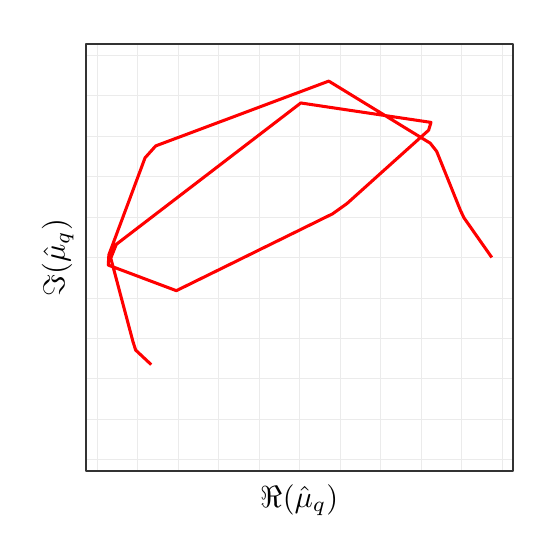
\begin{tikzpicture}[x=1pt,y=1pt]
\definecolor{fillColor}{RGB}{255,255,255}
\begin{scope}
\definecolor{drawColor}{RGB}{255,255,255}
\definecolor{fillColor}{RGB}{255,255,255}

\path[draw=drawColor,line width= 0.6pt,line join=round,line cap=round,fill=fillColor] (  0.00,  0.00) rectangle (180.67,180.68);
\end{scope}
\begin{scope}
\definecolor{fillColor}{RGB}{255,255,255}

\path[fill=fillColor] ( 20.71, 20.71) rectangle (175.17,175.17);
\definecolor{drawColor}{gray}{0.92}

\path[draw=drawColor,line width= 0.3pt,line join=round] ( 20.71, 24.81) --
	(175.17, 24.81);

\path[draw=drawColor,line width= 0.3pt,line join=round] ( 20.71, 54.06) --
	(175.17, 54.06);

\path[draw=drawColor,line width= 0.3pt,line join=round] ( 20.71, 83.32) --
	(175.17, 83.32);

\path[draw=drawColor,line width= 0.3pt,line join=round] ( 20.71,112.57) --
	(175.17,112.57);

\path[draw=drawColor,line width= 0.3pt,line join=round] ( 20.71,141.83) --
	(175.17,141.83);

\path[draw=drawColor,line width= 0.3pt,line join=round] ( 20.71,171.08) --
	(175.17,171.08);

\path[draw=drawColor,line width= 0.3pt,line join=round] ( 24.81, 20.71) --
	( 24.81,175.17);

\path[draw=drawColor,line width= 0.3pt,line join=round] ( 54.06, 20.71) --
	( 54.06,175.17);

\path[draw=drawColor,line width= 0.3pt,line join=round] ( 83.32, 20.71) --
	( 83.32,175.17);

\path[draw=drawColor,line width= 0.3pt,line join=round] (112.57, 20.71) --
	(112.57,175.17);

\path[draw=drawColor,line width= 0.3pt,line join=round] (141.83, 20.71) --
	(141.83,175.17);

\path[draw=drawColor,line width= 0.3pt,line join=round] (171.08, 20.71) --
	(171.08,175.17);

\path[draw=drawColor,line width= 0.6pt,line join=round] ( 20.71, 39.44) --
	(175.17, 39.44);

\path[draw=drawColor,line width= 0.6pt,line join=round] ( 20.71, 68.69) --
	(175.17, 68.69);

\path[draw=drawColor,line width= 0.6pt,line join=round] ( 20.71, 97.94) --
	(175.17, 97.94);

\path[draw=drawColor,line width= 0.6pt,line join=round] ( 20.71,127.20) --
	(175.17,127.20);

\path[draw=drawColor,line width= 0.6pt,line join=round] ( 20.71,156.45) --
	(175.17,156.45);

\path[draw=drawColor,line width= 0.6pt,line join=round] ( 39.44, 20.71) --
	( 39.44,175.17);

\path[draw=drawColor,line width= 0.6pt,line join=round] ( 68.69, 20.71) --
	( 68.69,175.17);

\path[draw=drawColor,line width= 0.6pt,line join=round] ( 97.94, 20.71) --
	( 97.94,175.17);

\path[draw=drawColor,line width= 0.6pt,line join=round] (127.20, 20.71) --
	(127.20,175.17);

\path[draw=drawColor,line width= 0.6pt,line join=round] (156.45, 20.71) --
	(156.45,175.17);
\definecolor{drawColor}{RGB}{255,0,0}

\path[draw=drawColor,line width= 1.1pt,line join=round] (167.40, 97.94) --
	(166.14, 99.74) --
	(164.88,101.54) --
	(163.62,103.33) --
	(162.36,105.13) --
	(161.10,106.92) --
	(159.85,108.72) --
	(158.59,110.51) --
	(157.33,112.31) --
	(156.09,114.94) --
	(154.86,117.99) --
	(153.63,121.04) --
	(152.41,124.09) --
	(151.18,127.13) --
	(149.95,130.18) --
	(148.72,133.23) --
	(147.49,136.28) --
	(145.15,139.25) --
	(140.57,142.05) --
	(135.99,144.85) --
	(131.41,147.66) --
	(126.83,150.46) --
	(122.24,153.26) --
	(117.66,156.06) --
	(113.08,158.87) --
	(108.50,161.67) --
	(100.68,158.74) --
	( 92.87,155.82) --
	( 85.05,152.89) --
	( 77.23,149.96) --
	( 69.41,147.03) --
	( 61.59,144.10) --
	( 53.78,141.18) --
	( 45.96,138.25) --
	( 42.11,133.94) --
	( 40.24,128.93) --
	( 38.37,123.93) --
	( 36.51,118.92) --
	( 34.64,113.92) --
	( 32.77,108.91) --
	( 30.91,103.91) --
	( 29.04, 98.90) --
	( 28.82, 95.18) --
	( 31.90, 94.03) --
	( 34.97, 92.87) --
	( 38.05, 91.72) --
	( 41.12, 90.56) --
	( 44.20, 89.40) --
	( 47.27, 88.25) --
	( 50.35, 87.09) --
	( 53.42, 85.94) --
	( 60.48, 89.41) --
	( 67.54, 92.88) --
	( 74.60, 96.35) --
	( 81.65, 99.83) --
	( 88.71,103.30) --
	( 95.77,106.77) --
	(102.82,110.24) --
	(109.88,113.72) --
	(115.05,117.40) --
	(119.27,121.19) --
	(123.49,124.98) --
	(127.70,128.77) --
	(131.92,132.56) --
	(136.14,136.35) --
	(140.36,140.14) --
	(144.58,143.93) --
	(145.43,146.75) --
	(139.55,147.63) --
	(133.67,148.50) --
	(127.79,149.38) --
	(121.91,150.26) --
	(116.03,151.13) --
	(110.15,152.01) --
	(104.27,152.89) --
	( 98.39,153.77) --
	( 90.06,147.38) --
	( 81.73,141.00) --
	( 73.40,134.62) --
	( 65.07,128.23) --
	( 56.74,121.85) --
	( 48.41,115.47) --
	( 40.08,109.09) --
	( 31.74,102.70) --
	( 29.73, 97.70) --
	( 30.87, 93.40) --
	( 32.02, 89.09) --
	( 33.16, 84.78) --
	( 34.30, 80.47) --
	( 35.45, 76.17) --
	( 36.59, 71.86) --
	( 37.74, 67.55) --
	( 38.73, 64.46) --
	( 39.43, 63.81) --
	( 40.13, 63.15) --
	( 40.83, 62.50) --
	( 41.53, 61.84) --
	( 42.23, 61.19) --
	( 42.93, 60.53) --
	( 43.63, 59.88) --
	( 44.33, 59.22);
\definecolor{drawColor}{gray}{0.20}

\path[draw=drawColor,line width= 0.6pt,line join=round,line cap=round] ( 20.71, 20.71) rectangle (175.17,175.17);
\end{scope}
\begin{scope}
\definecolor{drawColor}{RGB}{0,0,0}

\node[text=drawColor,anchor=base,inner sep=0pt, outer sep=0pt, scale=  1.10] at ( 97.94,  7.64) {$\Re(\hat\mu_q)$};
\end{scope}
\begin{scope}
\definecolor{drawColor}{RGB}{0,0,0}

\node[text=drawColor,rotate= 90.00,anchor=base,inner sep=0pt, outer sep=0pt, scale=  1.10] at ( 13.08, 97.94) {$\Im(\hat\mu_q)$};
\end{scope}
\end{tikzpicture}
